\documentclass[a4paper,12pt]{report}
\usepackage{graphicx}
\usepackage{array}
\graphicspath{{./images/}}
\begin{document}
	\begin{titlepage}
		\begin{center}
			
\includegraphics{ankara_bilim.png}
		\end{center}
		\vspace{1cm}
		\begin{center}
			\LARGE
			\textbf{SENG 244 - Object Oriented Software Engineering}
		\end{center}
		\vspace{1cm}
		\begin{center}
			\Large
			\textbf{Software Analysis Report}
		\end{center}
		\vspace{1cm}
		\begin{center}
			\Large
			\textbf{Non Governmental Organization - Aid Operations Management System}
		\end{center}
		\vspace{2cm}
		\begin{center}
			\large
			\textbf{BETG-4}
		\end{center}
		\vspace{1cm}
		\begin{center}
			\large
			Bora Eskin\\
			Eren Demir Özalban\\
			Talha Fatih Bülbül - 220204007\\
			Gürkan Köleoğlu
		\end{center}
	\end{titlepage}
	\tableofcontents
	\chapter{Introduction}
 		\paragraph{} Non-Governmental Organizations (NGOs) play a vital role in providing aid and support to communities worldwide, especially in regions affected by natural disasters, conflicts, and socio-economic challenges.
         	\paragraph{} To effectively manage their operations, NGOs rely on various systems and technologies, including Aid Operations Management Systems.
	  	\paragraph{} These systems streamline the processes involved in planning, executing, and monitoring aid activities, ensuring efficient resource allocation and delivery of services to those in need.
   		\paragraph{} This software analysis report aims to evaluate the current landscape of AOMS solutions utilized by NGOs, assessing their features, functionalities, strengths, and limitations. 
     		\paragraph{} By examining these aspects, we seek to provide insights into the effectiveness of existing systems and identify potential areas for improvement or innovation.
    
	\chapter{Overview (Domain Analysis)}
 		\paragraph{} Non-Governmental Organizations (NGOs) aid operations management systems include many different components. These components include donor, volunteer, needy, geographic information system (GIS), material aid, cash aid, and work breakdown structure (WBS).
		\paragraph{} These systems include a donor management component to track and manage the resources provided by donors. Likewise, volunteer management modules enable coordinating and tracking volunteers' contributions.
		\paragraph{} NGOs use systems to manage the information of the needy people they serve. This is important to monitor and improve the impact of services.
		\paragraph{} Geographic location is critical for planning aid distribution and analyzing impact. Therefore, geographic information systems (GIS) integration plays an important role in the effective management of relief operations.
		\paragraph{} NGOs use systems to effectively manage material and cash assistance. There are special modules for recording, monitoring and using these aids.
		\paragraph{} Finally, the work breakdown structure (WBS) is important for effective planning and management of aid projects. These structures define the parts of the project and ensure that resources are used effectively.
  
	\chapter{Functional Requirements}
	\begin{enumerate}
		\item Donors shall be able to register to the site.
		\item Donors shall be able to delete their account from the site.
		\item Donors shall be able to login to the site.
		\item Donors shall be able to logout from the site.
		\item The logged-in donors shall be able to select the area, project amount, and type of donation.
		
		\item Donors shall able to request shipment demand of their supply. The system give two choice to donor. Either donor can demand ship the item themselves or commend NGO to collect the item by specific time period.

		\item Volunteers shall be able to register on the site.
		
		\item Volunteers shall be able to delete their account from the site.
		\item Volunteers shall be able to login to the site.
		\item Volunteers shall be able to logout from the site.
		
		\item Volunteers shall have to construct a personal profile to register. The personal profile contains his/her profession, average annual income, geographical region they are willing to provide support to, transportation status, availability in terms of days within a month, and time interval.
		
		\item Volunteers shall be in the pending state after constructing the profile.
		
		\item The system Administrators shall have the authority to move any volunteers out of the pending state by accepting the profile.
		
		\item Indigent people shall have to apply for registration to find aid. This registration requires filling out a form that contains personal information of the indigent people, monthly income, number of people in the household, number of children, educational status of each child, employment status of the household members, monthly expenditures, and nature of support they need.
		
		\item Operation Coordinators shall be able to login to the site.
		\item Operation Coordinators shall be able to login to the site.
		\item Operation Coordinators shall be able to logout from the site.
		
		
		\item Operation Coordinators shall be able to schedule aid operations which involve collecting items from donors and shipping them to the warehouse.
		
		\item Operation Coordinators shall be able to schedule aid operations which involve shipping the aid items from the warehouse to people in need.
		
		\item  Operation Coordinators shall be able to schedule aid operations which involve organizing public events in case donations and/or volunteers drop below a certain threshold. They can do this by sending emails and SMS to registered and/or potential users to increase awareness.
		
		\item The system shall employ algorithms to analyze the current state of the donations.
		
		\item The system shall employ algorithms to analyze assistance requests.
		
		\item The system shall employ algorithms to analyze the availability of volunteers.
		
		\item The system shall employ algorithms to propose an optimum schedule for all requested operation types.
		
		\item The System Administrator shall be able to create registered users.
		
		\item The System Administrator shall be able to query registered users.
		
		\item The System Administrator shall be able to delete registered users.
		
		\item The System Administrator shall be able to see a dashboard where summary statistics will be displayed. 
		
		\item The System Administrator shall be able to see the number of new volunteers registered.
		
		\item The System Administrator shall be able to see the number of volunteers that left the system.
		\item The System Administrator shall be able to see the number of operations handled and their locations.
		
		\item The System Administrator shall be able to see the number of items left in the warehouse stock.
		
		
		
	\end{enumerate}
	\chapter{Nonfunctional Requirements}
	\section{Usability}
	\begin{enumerate}
		\item The user interface shall be active   user-friendly, allowing donors , volunteers and indigent people
		
		\item The user interface shall let to administrators to navigate the site easily.
		
		\item The system shall provide clear and simple  instructions for users how to logging in, selecting donations and and making a request for aid. 
		
		\item The system shall support main languages in and around national limits for improving accessibility and usability.
		
		\item The feedback mechanisms shall be adopted for the user interface to get feedback from users with their experience in the system.
	\end{enumerate}
	\section{Performance}
	\begin{enumerate}
		\item The system shall have fast response time  for user interactions. (Selecting donations , logging in)
		
		\item The system shall be able to handle a lot of users at the same time without noticeable performance decrease.
		
		\item Database shall be optimized for flexibility and effectiveness.
		
		\item The system architecture shall be designed effective for  memory, and storage capacity to control user demand.
		
		\item System caching mechanisms shall be implemented to reduce the needed space for repeated database 
	\end{enumerate}
	\section{Extensibility}
	\begin{enumerate}
		\item The system architecture shall be designed for allowing for upcoming updates and enchancements without requiring significant redevelopment.
		
		\item The system architecture shall be designed to support integration with third-party systems and services for the integration of new 
		functionalities and features.
		
		\item The system shall support  development/test scenarios for developers to experiment with new features and integrations before applying changes to the production environment.
		
		\item Documentation shall be presented for developers and system administrators,  for extending the system's functionality and integrating with outer systems.
		
		\item Continuous integration and deployment asset shall be authorized for the process of integrating and launching system extensions and improvements.
	\end{enumerate}
	\section{Others}
	\begin{enumerate}
		\item The system shall apply data protection regulations and privacy laws for user informations. 
		
		\item System documentation shall include user guides , technical guides. 
		
		\item The system shall have a high level of reliability
		
		\item Data encryption shall be used to protect sensitive and personal information.
		
		\item The system shall be well-documented, with detailed documentation covering system architecture, design decisions and develop techniques.
		
	\end{enumerate}
	
	\chapter{System Models}
	\section{Use Case Model}
		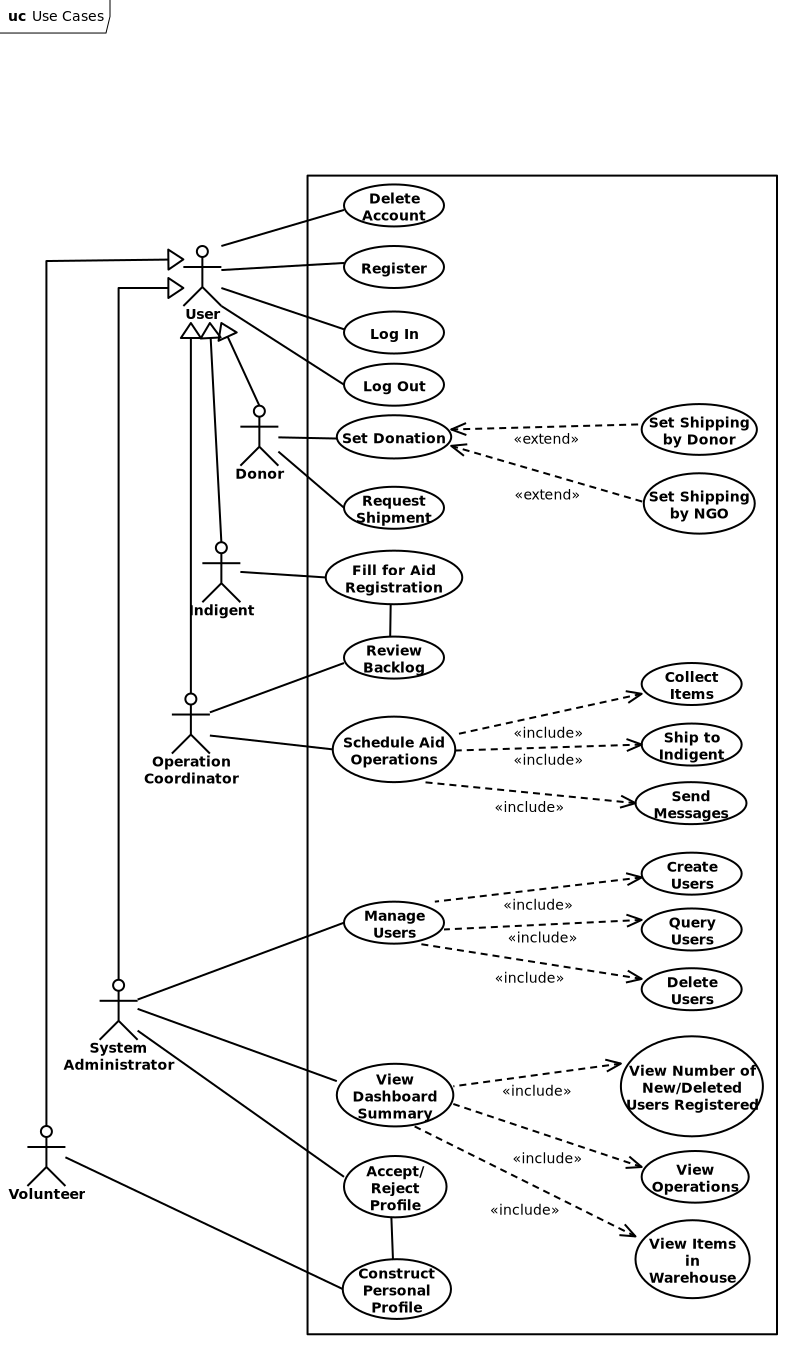
\includegraphics[width=216pt,height=351pt]{use_case_diagram.png} % width=8*27 pt,height= 13*27 pt
		\\ \\
		\begin{tabular}{|m{4cm}|m{11.5cm}|}
			\hline
					Use Case Name & Register\\
				\hline
					Use Case ID & 1\\
				\hline
					Primary System Actor & User\\
				\hline
					Participating Actor & -\\
				\hline
					Definition & An user registering to the system.\\
				\hline
					Precondition & The user opening the program.\\
				\hline
					Trigger & The user clicks on Register button.\\
				\hline
					Basic Path & \begin{enumerate}
						\item The user opens the program.
						\item The user clicks on Register button.
						\item The user enters their info.
						\item The user clicks okay.
						\item The user is signed up to the system.
					\end{enumerate}		
					\\
				\hline
					Alternative Path & -\\
				\hline
					Exceptional Case & \begin{enumerate}
						\item The user enters their info incorrectly.
						\item The system rejects the sign up.
						\item The system notifies the user of the rejection.
					\end{enumerate}
					
					\\
				\hline
					Postcondition & The user is signed up to the system.\\
				\hline
					Rules & -\\
				\hline
					Explanation & -\\
			\hline
		\end{tabular}
		\begin{tabular}{|m{4cm}|m{11.5cm}|}
			\hline
				Use Case Name & Log in\\
			\hline
				Use Case ID & 2\\
			\hline
				Primary System Actor & User\\
			\hline
				Participating Actor & -\\
			\hline
				Definition & An user logging into the system.\\
			\hline
				Precondition & The user has already signed up before.\\
			\hline
				Trigger & -\\
			\hline
				Basic Path & \begin{enumerate}
					\item The user opens the program.
					\item The user fills in necessary info to log in.
					\item The user clicks okay.
					\item The user is logged in to the system.
					\item The user is put into their respective menu.
				\end{enumerate}		
				\\
			\hline
				Alternative Path & -\\
			\hline
				Exceptional Case & \begin{enumerate}
					\item The user enters their info incorrectly.
					\item The system rejects the log in.
					\item The system notifies the user of the rejection.
				\end{enumerate}
				\\
			\hline
				Postcondition & The user is signed up to the system.\\
			\hline
				Rules & -\\
			\hline
				Explanation & -\\
			\hline
		\end{tabular}
		\begin{tabular}{|m{4cm}|m{11.5cm}|}
			\hline
				Use Case Name & Log Out\\
			\hline
				Use Case ID & 3\\
			\hline
				Primary System Actor & User\\
			\hline
				Participating Actor & -\\
			\hline
				Definition & An user logging out of the system.\\
			\hline
				Precondition & The user is logged in currently.\\
			\hline
				Trigger & \\
			\hline
				Basic Path & \begin{enumerate}
					\item The user clicks the log out button.
					\item The system logs user out.
					\item The user is put back into log in menu.
				\end{enumerate}		
				\\
			\hline
				Alternative Path & -\\
			\hline
				Exceptional Case & -\\
			\hline
				Postcondition & The user is logged out of the system.\\
			\hline
				Rules & -\\
			\hline
				Explanation & -\\
			\hline
		\end{tabular}
		\begin{tabular}{|m{4cm}|m{11.5cm}|}
			\hline
				Use Case Name & Set Donation\\
			\hline
				Use Case ID & 4\\
			\hline
				Primary System Actor & User\\
			\hline
				Participating Actor & -\\
			\hline
				Definition & A donor setting a donation request.\\
			\hline
				Precondition & The donor is logged in currently.\\
			\hline
				Trigger & -\\
			\hline
				Basic Path & \begin{enumerate}
					\item The donor clicks the set donation button.
					\item A new page opens where you can enter info needed for setting a donation.
					\item The donor enters necessary information.
					\item The donor clicks okay.
					\item The donation request is saved.
					\item The system puts the donor back to the main menu.
				\end{enumerate}		
				\\
			\hline
				Alternative Path & -\\
			\hline
				Exceptional Case & \begin{enumerate}
					\item The donor doesn't fill required info incomplete.
					\item The system rejects the creation of donation.
					\item The system notifies the user of the rejection with what part is missing.
				\end{enumerate}
				\\
			\hline
				Postcondition & -\\
			\hline
				Rules & -\\
			\hline
				Explanation & -\\
			\hline
		\end{tabular}
		\begin{tabular}{|m{4cm}|m{11.5cm}|}
			\hline
				Use Case Name & Request Shipment\\
			\hline
				Use Case ID & 5\\
			\hline
				Primary System Actor & Donor\\
			\hline
				Participating Actor & -\\
			\hline
				Definition & A donor sending a request for their donations to be sent.\\
			\hline
				Precondition & The donor is logged in currently and has a set donation.\\
			\hline
				Trigger & -\\
			\hline
				Basic Path & \begin{enumerate}
					\item The Donor opens their donations.
					\item The Donor selects the request shipment option for the donation.
					\item The system sends a request for shipment.
					\item The system confirms their request has been sent.
				\end{enumerate}		
				\\
			\hline
				Alternative Path & -\\
			\hline
				Exceptional Case & -\\
			\hline
				Postcondition & -\\
			\hline
				Rules & -\\
			\hline
				Explanation & -\\
			\hline
		\end{tabular}
		\begin{tabular}{|m{4cm}|m{11.5cm}|}
			\hline
				Use Case Name & Fill for Aid Registration\\
			\hline
				Use Case ID & 6\\
			\hline
				Primary System Actor & Indigent\\
			\hline
				Participating Actor & -\\
			\hline
				Definition & An indigent sending a form to be evaluated their indigent status.\\
			\hline
				Precondition & -\\
			\hline
				Trigger & -\\
			\hline
				Basic Path & \begin{enumerate}
					\item The indigent opens the system.
					\item The indigent selects the Fill for Aid registration button.
					\item The system opens a form for Aid Registration.
					\item The indigent fills the form.
					\item The indigent clicks the okay button.
					\item The system accepts the form and saves it.
					\item The system indicates the form has been accepted to the user.
					\item The system puts the user back in the log in menu.
				\end{enumerate}		
				\\
			\hline
				Alternative Path & -\\
			\hline
				Exceptional Case & \begin{enumerate}
					\item The indigent leaves some blanks in the form.
					\item The indigent clicks the okay button.
					\item The system rejects the form as a result.
					\item The system indicates the form has been rejected to the user.
				\end{enumerate}
				\\
			\hline
				Postcondition & -\\
			\hline
				Rules & -\\
			\hline
				Explanation & -\\
			\hline
		\end{tabular}
		\begin{tabular}{|m{4cm}|m{11.5cm}|}
			\hline
				Use Case Name & Review Backlog\\
			\hline
				Use Case ID & 7\\
			\hline
				Primary System Actor & Operation Coordinator\\
			\hline
				Participating Actor & -\\
			\hline
				Definition & Allow an Operation Coordinator to see a backlog.\\
			\hline
				Precondition & The Operation Coordinator is logged in.\\
			\hline
				Trigger & -\\
			\hline
				Basic Path & \begin{enumerate}
					\item The Operation Coordinator clicks on the Review Backlog button.
					\item The System shows related info to the Review Backlog.
					\item The Operation Coordinator checks the info as long as needed by them.
					\item The Operation Coordinator clicks the back button.
					\item The System puts the Operation Coordinator back to the main menu.
				\end{enumerate}		
				\\
			\hline
				Alternative Path & -\\
			\hline
				Exceptional Case & -\\
			\hline
				Postcondition & -\\
			\hline
				Rules & -\\
			\hline
				Explanation & -\\
			\hline
		\end{tabular}
		\begin{tabular}{|m{4cm}|m{11.5cm}|}
			\hline
				Use Case Name & Schedule Aid Operation\\
			\hline
				Use Case ID & 8\\
			\hline
				Primary System Actor & Operation Coordinator\\
			\hline
				Participating Actor & -\\
			\hline
				Definition & An Operation Coordinator scheduling an operation.\\
			\hline
				Precondition & The Operation Coordinator is logged in.\\
			\hline
				Trigger & -\\
			\hline
				Basic Path & \begin{enumerate}
					\item The Operation Coordinator clicks on Schedule Aid Operation button.
					\item The Operation Coordinator chooses between three operation types: Collect Items from Donors to the Warehouse, Ship Items to the Indigent from the Warehouse and Raising Awareness by Sending Messages.
					\item The Operation Coordinator fills related info for the selected operation.
					\item The Operation Coordinator clicks the okay button.
					\item The System saves the form.
					\item The System notifies the Operation Coordinator of the confirmation.
					\item The System puts the Operation Coordinator back to the main menu.
				\end{enumerate}		
				\\
			\hline
				Alternative Path & -\\
			\hline
				Exceptional Case & \begin{enumerate}
					\item The Operation Coordinator fills related info wrongly.
					\item The Operation Coordinator clicks the okay button.
					\item The System rejects the form.
					\item The System notifies the Operation Coordinator of the rejection with related info.
					\item The System puts the Operation Coordinator back to the form.
				\end{enumerate}
				\\
			\hline
				Postcondition & -\\
			\hline
				Rules & -\\
			\hline
				Explanation & -\\
			\hline
		\end{tabular}
		\begin{tabular}{|m{4cm}|m{11.5cm}|}
			\hline
				Use Case Name & Manage Users\\
			\hline
				Use Case ID & 9\\
			\hline
				Primary System Actor & System Administrator\\
			\hline
				Participating Actor & -\\
			\hline
				Definition & A system administrator managing the users inside the system.\\
			\hline
				Precondition & The System Administrator is logged in.\\
			\hline
				Trigger & -\\
			\hline
				Basic Path & \begin{enumerate}
					\item The System Administrator clicks the Manage Users button.
					\item The System gives a list of existing users.
					\item The System Administrator chooses one of the ways to manage a user. The options include: Create User, Query User, Delete User.
					\item The System Administrator fills necessary information.
					\item The System Administrator clicks the okay button.
					\item The System does the requested change.
					\item The System notifies the user of the completed change.
				\end{enumerate}		
				\\
			\hline
				Alternative Path & -\\
			\hline
				Exceptional Case & -\\
			\hline
				Postcondition & -\\
			\hline
				Rules & -\\
			\hline
				Explanation & -\\
			\hline
		\end{tabular}
		\begin{tabular}{|m{4cm}|m{11.5cm}|}
			\hline
				Use Case Name & View Dashboard Summary\\
			\hline
				Use Case ID & 10\\
			\hline
				Primary System Actor & System Administrator\\
			\hline
				Participating Actor & -\\
			\hline
				Definition & A system administrator viewing a dashboard \\
			\hline
				Precondition & The System Administrator is logged in.\\
			\hline
				Trigger & -\\
			\hline
				Basic Path & \begin{enumerate}
					\item The System Administrator clicks the Manage Users button.
					\item The System gives a list of existing users.
					\item The System Administrator chooses one of the ways to manage a user. The options include: Create User, Query User, Delete User.
					\item The System Administrator fills necessary information.
					\item The System Administrator clicks the okay button.
					\item The System does the requested change.
					\item The System notifies the user of the completed change.
				\end{enumerate}		
				\\
			\hline
				Alternative Path & -\\
			\hline
				Exceptional Case & -\\
			\hline
				Postcondition & -\\
			\hline
				Rules & -\\
			\hline
				Explanation & -\\
			\hline
		\end{tabular}
		\begin{tabular}{|m{4cm}|m{11.5cm}|}
			\hline
				Use Case Name & Accept/Reject Profile\\
			\hline
				Use Case ID & 11\\
			\hline
				Primary System Actor & System Administrator\\
			\hline
				Participating Actor & -\\
			\hline
				Definition & A system administrator accepting the profile of a volunteer.\\
			\hline
				Precondition & The System Administrator is logged in.\\
			\hline
				Trigger & -\\
			\hline
				Basic Path & \begin{enumerate}
					\item The System Administrator clicks the View Volunteer Profiles button.
					\item The System views a list of Volunteer Profiles.
					\item The System Administrator clicks on one of the Volunteer Profiles.
					\item The System shows the chosen Volunteer Profile.
					\item The System Administrator checks the profile as long as needed.
					\item The System Administrator either accepts or rejects the profile.
					\item The System sets the status of the profile to either accepted or rejected.
					\item The System notifies either of acceptance or rejection of the profile.
					\item The System puts the System Administrator back to the list of Volunteer Profiles.
				\end{enumerate}		
				\\
			\hline
				Alternative Path & -\\
			\hline
				Exceptional Case & -\\
			\hline
				Postcondition & -\\
			\hline
				Rules & -\\
			\hline
				Explanation & -\\
			\hline
		\end{tabular}
		\begin{tabular}{|m{4cm}|m{11.5cm}|}
			\hline
				Use Case Name & Construct Personal Profile\\
			\hline
				Use Case ID & 12\\
			\hline
				Primary System Actor & Volunteer\\
			\hline
				Participating Actor & -\\
			\hline
				Definition & A system administrator accepting the profile of a volunteer.\\
			\hline
				Precondition & The System Administrator is logged in.\\
			\hline
				Trigger & -\\
			\hline
				Basic Path & \begin{enumerate}
					\item The System Administrator clicks the View Volunteer Profiles button.
					\item The System views a list of Volunteer Profiles.
					\item The System Administrator clicks on one of the Volunteer Profiles.
					\item The System shows the chosen Volunteer Profile.
					\item The System Administrator checks the profile as long as needed.
					\item The System Administrator either accepts or rejects the profile.
					\item The System sets the status of the profile to either accepted or rejected.
					\item The System notifies either of acceptance or rejection of the profile.
					\item The System puts the System Administrator back to the list of Volunteer Profiles.
				\end{enumerate}		
				\\
			\hline
				Alternative Path & -\\
			\hline
				Exceptional Case & -\\
			\hline
				Postcondition & -\\
			\hline
				Rules & -\\
			\hline
				Explanation & -\\
			\hline
		\end{tabular}
	\section{Dynamic Models}
	\section{Object and Class Model}
	\section{Sequence Diagram}
	\section{User Interfaces}
	\section{Glossary and References}
\end{document}
